\section{A Primer on Spuriousness (Real/Bogus)}\label{sec:rb}

The completeness, purity, and spuriousness of samples of detected sources are all related to detection efficiencies. 

When source detection is performed on a difference image, both true astrophysical sources and artifact sources can be detected with $SNR > {transSNR} = 5$ and become {\tt DIASources}.
Examples of artifacts include, e.g., sources caused by telescope hardware, or incompletely removed cosmic rays (despite the fact that cosmic rays are real astrophysical messengers). 

{\bf Spuriousness ($\mathcal{S}$):} a parameter, typically between $0$ and $1$, which represents the probability that a source is astrophysical (values closer to $1$) or artifact (values closer to $0$).

The spuriousness is sometimes also called the {\it real/bogus score}.
It is typically determined by machine learning on many sources that were pre-classified as astrophysical (real) or artifact (bogus), and usually considers factors like the shape of the point source in the difference image (e.g., symmetry, sharpness). 

{\bf Spuriousness Threshold ($\tau_{\mathcal{S}}$):} a lower limit on spuriousness, $\mathcal{S}$, which can be applied to {\tt DIASources} to separate the "real" from the "bogus", and to thereby obtain a subset of {\tt DIASources} with a lower fraction of artifacts. 

The following definitions describe the classification of detected {\tt DIASources}, which were either truly real (astrophysical source) or truly false (artifact), as real or bogus by an applied spuriousness threshold $\tau_{\mathcal{S}}$:

\begin{tabular}{rl}
True Positive ($\mathit{TP}$) & A detected astrophysical source that was classified as real. \\
False Positive ($\mathit{FP}$) & A detected artifact that was classified as real. \\
True Negative ($\mathit{TN}$) & A detected artifact that was classified as bogus. \\
False Negative ($\mathit{FN}$) & A detected astrophysical source that was classified as bogus. \\
\end{tabular}

{\bf Completeness ($\mathcal{C}$):} the fraction of all detected astrophysical sources which are classified as real. This is also called the true positive rate, $\mathit{TPR} = \frac{\mathit{TP}}{\mathit{TP}+\mathit{FN}}$.

{\bf Purity ($\mathcal{P}$):} the fraction of all detected sources that were classified as real which are astrophysical in nature: $\frac{\mathit{TP}}{\mathit{TP}+\mathit{FP}}$. This is also called the {\it precision} or the {\it positive predictive value} ($\mathit{PPV}$) of a survey. 

The false positive rate\footnote{Note that in some published literature the false positive rate is instead defined as the fraction of all detected artifacts that were classified as real, $\mathit{FPR} = \frac{\mathit{FP}}{\mathit{TN}+\mathit{FP}}$.} is the fraction of all detected sources that were classified as real but which are artifacts: $\mathit{FPR} = 1 - \mathit{PPV} = \frac{\mathit{FP}}{\mathit{TP}+\mathit{FP}}$.

The relationship between the completeness and purity of a sample of {\tt DIASources} classified as real can be traced out by varying $\tau_{\mathcal{S}}$.

In Figure \ref{fig:comp_pure} we show, as an example, the relationship between the false positive rate ($\mathit{FPR}$; purity) and the missed detection rate ($\mathit{MDR}$; completeness) for different types of source classification (i.e., real/bogus) algorithms from the Palomar Transient Factory \citep[PTF;][]{2013MNRAS.435.1047B}.
This relationship is formally known as the Receiver Operating Characteristic (ROC) curve when it is plotted as the true positive rate {\it vs.} the false positive rate for a given {\tt transSNR}.

\begin{figure}
\begin{center}
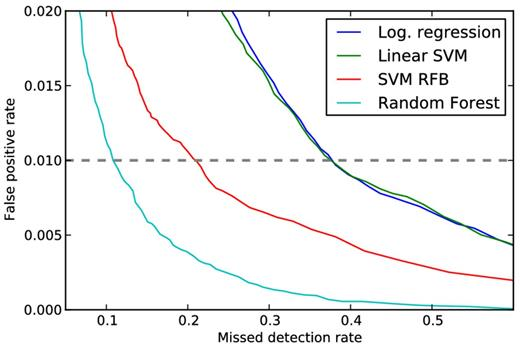
\includegraphics[width=8cm,trim={0cm 0cm 0cm 0cm}, clip]{figures/Brink_etal_2013_Fig3.jpg}
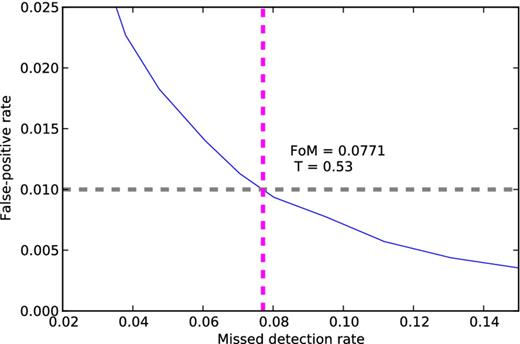
\includegraphics[width=8cm,trim={0cm 0cm 0cm 0cm}, clip]{figures/Brink_etal_2013_Fig7.jpg}
\caption{{\it Left:} An example of the relationship between the false positive rate ($\mathit{FPR}$; purity) {\it vs.} the missed detection rate ($\mathit{MDR}$; completeness) for different types of source classification (real/bogus) algorithms considered by the Palomar Transient Factory \citep{2013MNRAS.435.1047B}. {\it Right:} The relationship between $\mathit{FPR}$ and $\mathit{MDR}$ for the RB2 (real-bogus version 2) classifier (blue line) developed by the PTF and introduced in \cite{2013MNRAS.435.1047B}. Dashed lines show how $\mathit{FPR}=0.01$ is achieved with a spuriousness (real-bogus score value) threshold of $\tau=0.53$, which results in $\mathit{MDR}=0.077$. \label{fig:comp_pure}}
\end{center}
\end{figure}

{\bf Characterizing spuriousness} requires knowing which of the detected {\tt DIASources} are astrophysical (truly real) and which are artifacts (truly bogus).
Synthetic source injection is best for simulating astrophysical (real) sources because artifacts (bogus) can be a very diverse group; source injection cannot reveal which {\tt DIASources} in an image are artifacts.
Instead, characterizing spuriousness is achieved by building a training set of point sources that have been confirmed as astrophysical and artifact, using that training set for the spuriousness ($\mathcal{S}$; real/bogus) assignments by the machine learning algorithm.
Then, since ${transSNR}\propto m$, the ROC curve yields $\mathcal{C}(m,\tau_{\mathcal{S}})$ and $\mathcal{P}(m,\tau_{\mathcal{S}})$.
